\chapter{Experimental Results and Evaluations}
\label{chap:k3}

\cref{sec:Materials} provides information about input dataset and the applied preprocessing steps. 

evaluation procedure
%The distance between the LIDAR points and the generated DSM are computed and evaluated statistically
%To evaluate the influence of the over-counting correction and MGM
%cost aggregation independently, two evaluations were performed


In \cref{sec:sd}, the correctness of the derived model is firstly verified by using simulation data without adding errors in the simulated measurements yet some biases are added in the initial values of the unknowns.

Dashed lane-lines reconstruction is presented in \cref{sec:td-short}. % 5 set of dashed lane line data
% show the differences with DSM profile
In long lane-lines reconstruction cases

%%%%%%%%%%%%%%%%%%%%%%%%%%%%%%%%%%%%%%%%%%%%%%%%%%%%%%%%
\section{Materials}
\label{sec:Materials}

\paragraph{Aerial Images}
For real-time mapping applications during disasters, mass events and traffic monitoring scenarios, the German Aerospace Center (DLR) has developed a new optical sensor system-- the 4k system-- on a helicopter from DLR. The oblique aerial images used in this work are acquired from a Canon EOS 1D-X camera, one of the three non-metric cameras in the 4k system, with an oblique viewing angle $\tau$ of 15$\degree$. The image data sets used in this work were acquired in around 500m flying height $H_{flight height}$ above ground, which leads to a GSD of ~7cm. % data of acquisition, number of images, length of flight strips,…->maybe in chapter “Experiments?

An example aerial image is shown in \cref{fig:OriImg}. \cref{tab:CameraProperties} lists the properties of this camera, and \cref{tab:SensorViewingGeometry} provides the viewing geometry information.


\begin{table}%[!h]
  \centering
  \begin{tabular}{ll}
  \toprule
                                      {} & \textbf{Canon EOS 1D-X} \\
  \midrule
  Lenses                          & Zeiss Makro Planar 2/50\\
  \\[-1em]
  Sensor / Pixel size             & Full frame CMOS / 6.944 \textmu m\\
  \\[-1em]
  \multirow{2}{*}{Image size}     & 5184$\times$3456 pixel, ratio 3:2\\
                                  & (17.9 MPix)\\
  \\[-1em]
  ISO                             & 100--204800\\
  \\[-1em]
  max. frame rate / max. images   & 14 fps/ 180 images\\
  \\[-1em]
  Exposure time                   & 30 s -- 1/8000 s\\
  \\[-1em]
  Data interface                  & LAN (EDSDK software interface)\\
  \bottomrule
  \end{tabular}
  \caption{Properties of the oblique camera }
  \label{tab:CameraProperties}
%\end{table}
\vspace{1cm}
%\begin{table}%[!h]
  \centering
  \begin{tabular}{lll}
  \toprule
                         & \textbf{RGB, 50mm lens} \\
  \midrule
  Viewing directions     & $\pm$15$\degree$\\
  \\[-1em]
  \multirow{2}{*}{FOV}   & $\pm$34$\degree$ across strip,\\
                         & $\pm$13$\degree$ along strip\\
  \\[-1em]
  Coverage @500m         & 780 m $\times$ 230 m\\
  GSD      @500m         & 6.9 cm (nadir)\\

  \bottomrule
  \end{tabular}
  \caption{Viewing geometry}
  \label{tab:SensorViewingGeometry}
\end{table}

The images used in this work are acquired with a special flight configuration at both sides of the motorway which guarantees a continuous stereo view perpendicular to the lane marking direction.\footnote{The classical photogrammetric approach on flight planning is to have several straight flight lines which cover the whole motorway in a stereo view. This would be possible in this project yet would require more flight costs and would produce many more images.} This is realized by flying at the right-hand side with respect to flying direction along the motorway, with the left oblique camera looking left-down to the motorway, in both forward and backward trip. The flight configuration is shown in \cref{fig:FlightTrajectory} on the Google Earth platform.

Besides, the forward overlap is around 70\%, and all the lane markings are covered by both strips, whereas the side overlap depends on the distance of flight strips, which are a result of the pilots navigation ability and other influences, like wind. Nevertheless, the motorway in its entire width was covered by the two flight strips. Altogether, this results in approximately 8-image coverage in road areas. 

\begin{figure}%[!h]
  \centering
  \subfloat[]{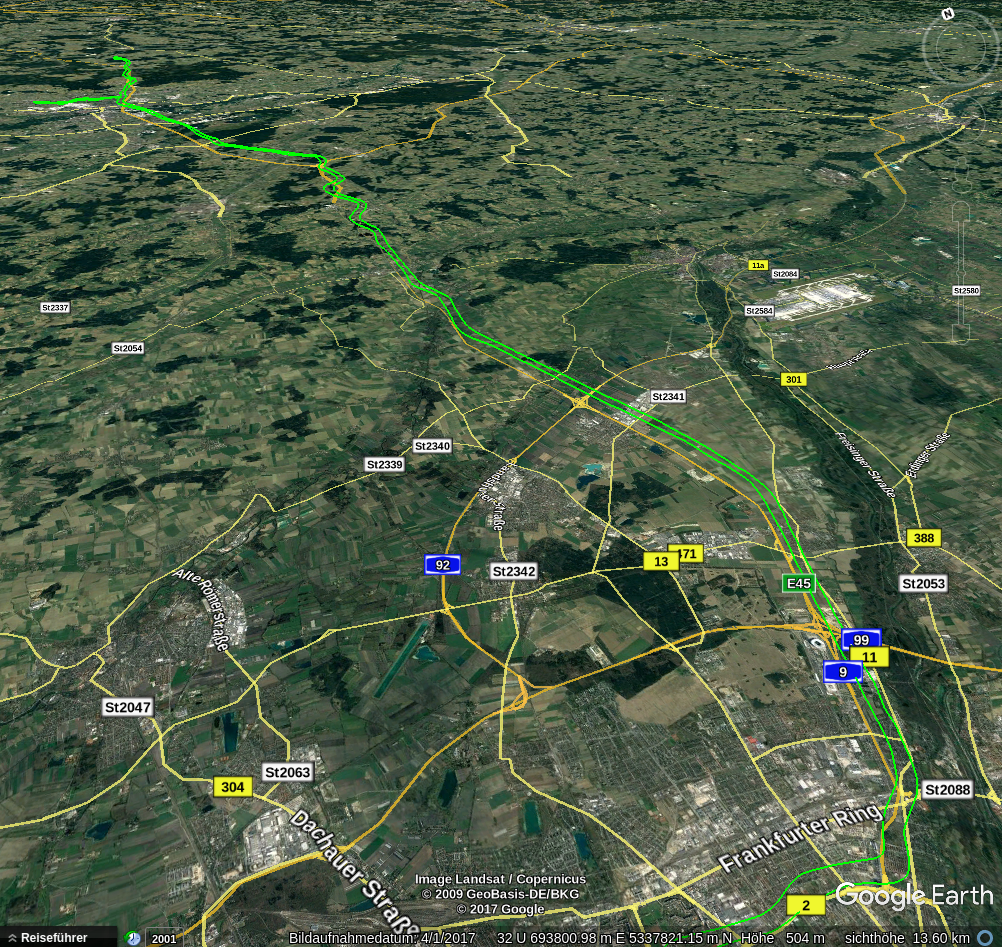
\includegraphics[height=0.45\textwidth]{FlightTrajectory5.png} \label{fig:trajectory1}}
  \subfloat[]{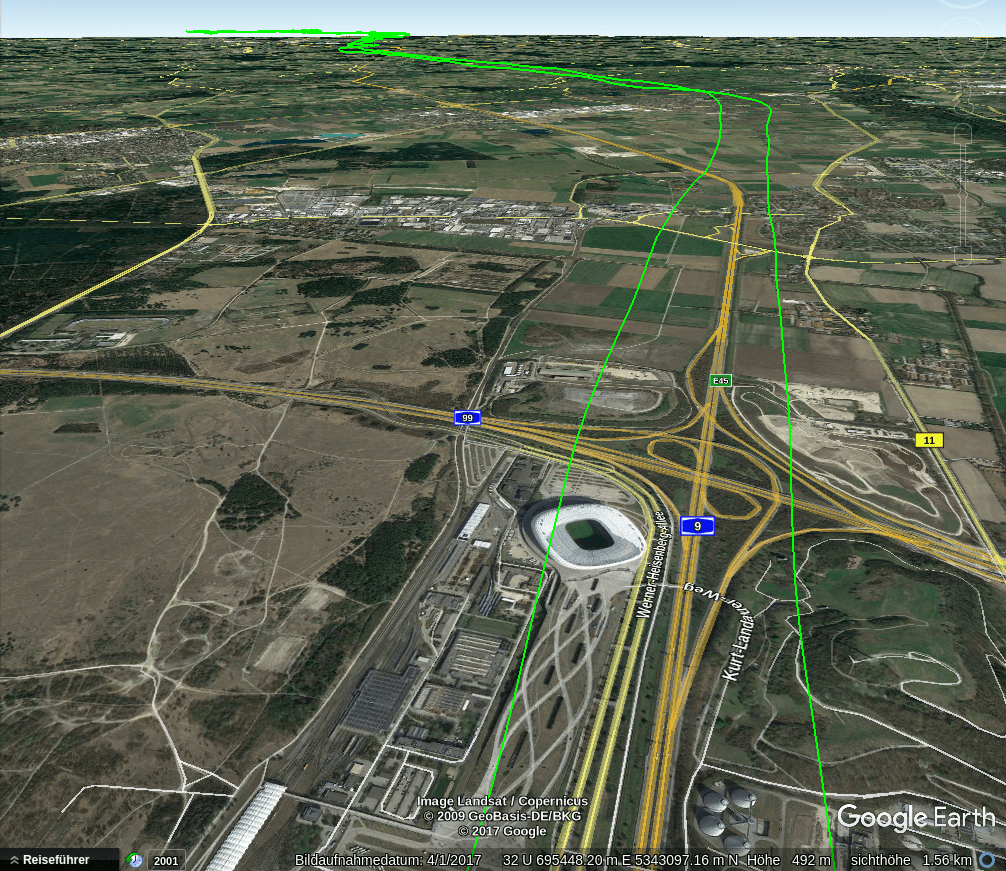
\includegraphics[height=0.45\textwidth]{FlightTrajectory3.png} \label{fig:trajectory2}}
  \caption{\small Flight trajectory of DLR helicopter visualized on the Google Earth platform. The green polyline shows the flight trajectory. \textit{Source: \textbf{Google Earth} 04/01/2017}}
  \label{fig:FlightTrajectory}
\end{figure}


\paragraph{Exterior and Interior Orientations}
The \gls{eo} of the images are directly measured by a GNSS/Inertial system IGI IId.% Missing: specification of the system, improvements by SAPOS correction,….
The EO parameters are then refined by a self-calibrating bundle adjustment. The accuracies of the exterior orientation (EO) parameters are shown in \cref{tab:EOaccuracy}. The calibrated \gls{io} parameters and their accuracies are shown in \cref{tab:IOaccuracy}. To provide an overall quality on the interior orientations: from the calibration result of interior orientations (involving lens distortion), the residuals appear non-systematic and the biggest residual $r_{max, IO}$ is around $1$ pixel.

To judge the influence of exterior and interior parameters on positioning accuracy in object space, the maximum values for each component based on the flight configuration was calculated.
The quality of interior and exterior orientation parameters set would have a maximum impact in object space for around $16.5$ [cm] in X,Y-direction:
\begin{itemize}
      \item caused by inaccurate camera position: 
      \item [] $\sqrt{\sigma_{north}^2+\sigma_{east}^2}=\sqrt{0.055^2+0.035^2}\approx0.065$ [meter]
      \item caused by inaccurate camera attitude:
      \item [] $\tan(\sqrt{\sigma_{roll}^2+\sigma_{pitch}^2})\times H_{flight height}\times\dfrac{1}{\cos^2\tau}$
      \item [] $=\tan(\sqrt{0.002^2+0.002^2})\times 500\times\dfrac{1}{\cos^215\degree}\approx0.026$ [meter]
      \item caused by inaccurate Interior Orientations:
      \item [] $r_{max, IO}\times GSD\times\dfrac{1}{\cos^2\tau}=1\times0.069\times\dfrac{1}{\cos^215\degree}\approx0.074$ [meter]
\end{itemize}
and around $9.4$ [cm] in Z-direction:
\begin{itemize}
      \item caused by inaccurate camera position:
      \item [] $\sigma_{altitude}\approx0.069$ [meter]
      \item caused by inaccurate camera attitude:
      \item [] $\tan(\sqrt{\sigma_{roll}^2+\sigma_{pitch}^2})\times H_{flight height}\times\dfrac{\sin\tau}{\cos\tau}$
      \item [] $=\tan(\sqrt{0.002^2+0.002^2})\times 500\times\dfrac{\sin15\degree}{\cos15\degree}\approx0.007$ [meter]
      \item caused by inaccurate Interior Orientations:
      \item [] $r_{max, IO}\times GSD\times\dfrac{\sin\tau}{\cos\tau}=1\times0.069\times\dfrac{\sin15\degree}{\cos15\degree}\approx0.018$ [meter]
\end{itemize}

The above information tells the positioning accuracy in object space with measurements on a single image. With corresponding measurements from multiple stereo views, which allows the intersection of multiple  rays, the positioning accuracy is expected to be improved for being overdetermined.

\begin{table}%[!h]
    \centering
    \begin{tabular}{ll|ll}
    \toprule
    position accuracies  &[meter]  & attitude accuracies & [degree]\\
    \midrule
    $\sigma_{north}$     & $0.055$ & $\sigma_{Roll}$  & $0.002$\\
    $\sigma_{east}$      & $0.035$ & $\sigma_{Pitch}$ & $0.002$\\
    $\sigma_{altitude}$  & $0.069$ & $\sigma_{Yaw}$   & $0.005$\\
    \bottomrule
    \end{tabular}
    \caption{Accuracies of Exterior Orientations}
    \label{tab:EOaccuracy}
%\end{table}
\vspace{1cm}
%\begin{table}%[!h]
    \centering
    \begin{tabular}{lr|lr|l}
    \toprule
    \multicolumn{2}{c|}{Interior Orientations}  & \multicolumn{2}{c|}{accuracies} & unit\\
    \midrule
    focal length $c$                       &   $0.051$ & $\sigma_c$      & $6.9\mathrm{e}{-7}$ & [meter]\\
    x coordinate of principal point $pp_x$ & $-42.259$ & $\sigma_{pp_x}$ & $0.167$             &[$\mu$m]\\
    x coordinate of principal point $pp_y$ & $115.384$ & $\sigma_{pp_y}$ & $0.799$             &[$\mu$m]\\
    \bottomrule
    \end{tabular}
    \caption{Interior Orientations and their accuracies}
    \label{tab:IOaccuracy}
\end{table}

\paragraph{\gls{dsm}}
For each pair of stereo images, a disparity map is generated using \gls{sgm} algorithm. With disparity's property of being inversely proportional to depth, the disparity maps can be used to derive the DSM. Since SGM is a kind of appearance-based matching, the SGM-generated DSM is noisy in lowly textured regions. 
%In most of the cases, a point in object space is covered by more than two aerial images, resulting in more than one disparity map. This leads to ambiguities on height decision during DSM generations.
%, and can be solved by simply taking the median value derived from disparity maps in odd number of disparity maps cases, and the value just lower than the median in even number cases. %This results in systematic errors of having lower height value in some parts of DSM.(The whole proof of this sentence is more complicated, I hope you will be not asked about this.)
Thus, the DSM will be used only for setting up the initial values of the work flow, and will not influence the final results of the 3D lane marking reconstruction.

The DSM has 20 cm grid spacing. \cref{fig:DSM} shows a part of the DSM. Standard deviations of the height value in this part of the DSM is shown in \cref{fig:DSMstd}. The number of stereo image pairs used for each part on the DSM is shown in \cref{fig:DSMnumber}.
% problem of higher noise at road surfaces
% Standard deviation not well visible. Maybe add number of images for this small part
\begin{figure}%[!h]
  \centering
  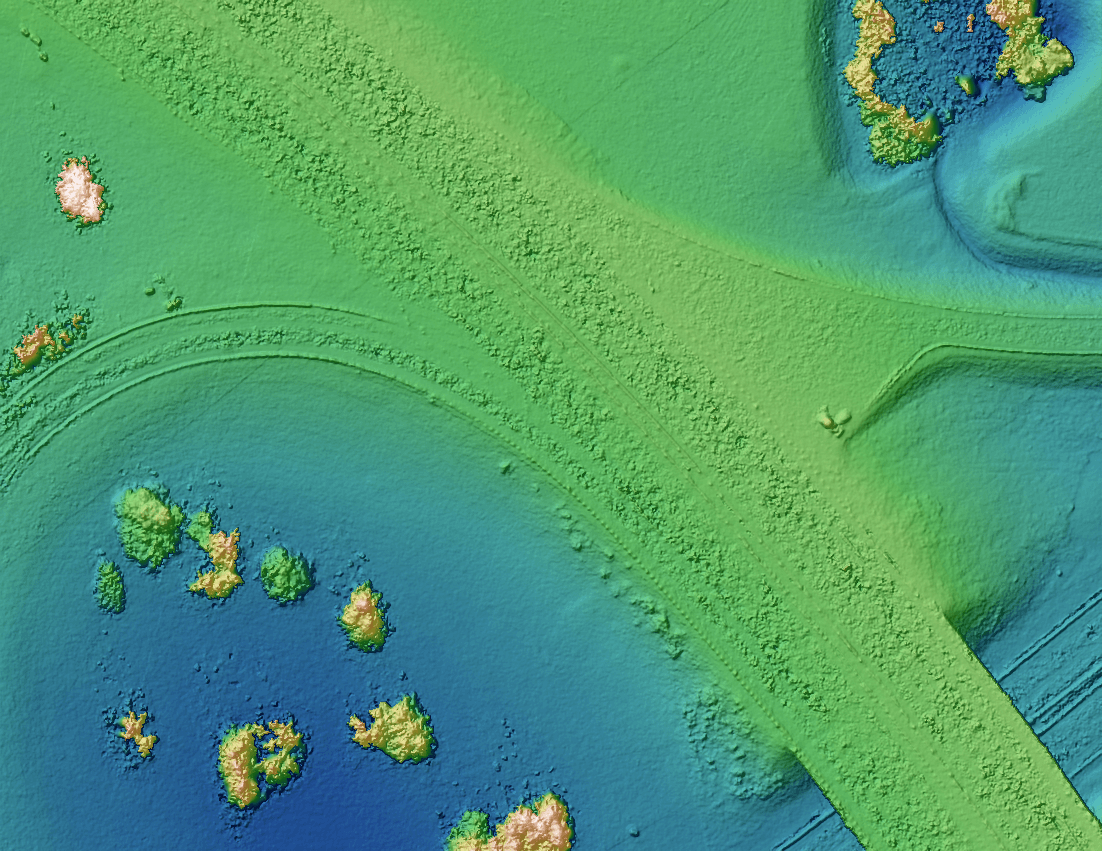
\includegraphics[width=0.8\textwidth]{DEM_A9_FINAL_PART_small_shaded.png}
  \caption{\small Part of the DSM in road area. It is noisy in the center of motorway.}
  \label{fig:DSM}
  \vspace{1cm}
  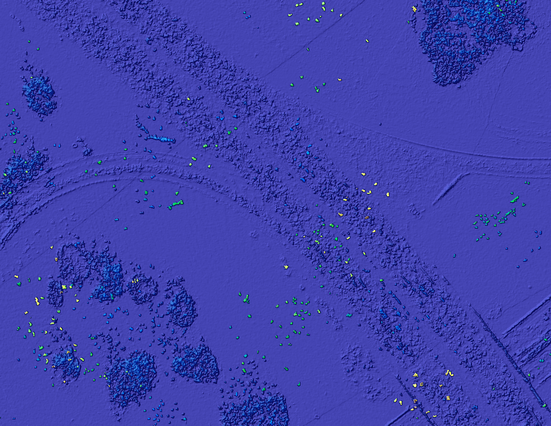
\includegraphics[width=0.8\textwidth]{DEM_A9_STD_small_terrain.png}
  \caption{\small Standard deviations of the height value of the DSM in road area. It has higher value in the center of motorway.}
  \label{fig:DSMstd}

\end{figure}

\begin{figure}%[!h]
  \centering
  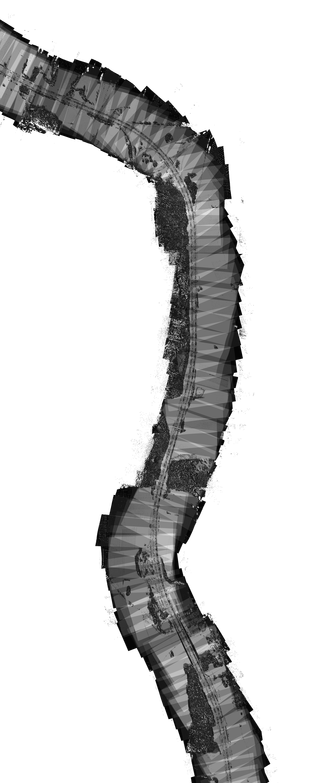
\includegraphics[width=0.5\textwidth]{DEM_A9_NUM_scaled_s.png}
  \caption{\small Distribution of stereo pairs used for DSM generation. Lighter color indicates more stereo pairs are used in that area. Maximum 27 stereo pairs are used for one pixel.}%%%%%%%%
  \label{fig:DSMnumber}
\end{figure}


\paragraph{Orthorectified Images}
The orthorectified images are processed using the DSM and the interior and exterior orientations derived from the bundle adjustment. They are georeferenced and the scale is uniform. One of the orthorectified images is shown in \cref{fig:OrthoImg}. The orthorectified images are only used for setting up initial values and used as intermediary step for processing the road masks, but do not influence the results of 3D lane marking reconstruction.
% Maybe a nice place, to visualize the DSM error on the lane marking projections…

\paragraph{Road Masks}
Road segments are masked out from original images based on \gls{osm} data: Firstly, the rasterized road segments from OSM data are written with 25 meter buffer width around road axes into orthorectified images. By back-projecting the mask from orthorectified image to original image using the 3D information from the DSM, it can then be used to mask out the road regions on the original images, as shown in \cref{fig:MaskedImg}.

\begin{figure}%[!h]
  \parbox{.475\linewidth}{
    \centering
    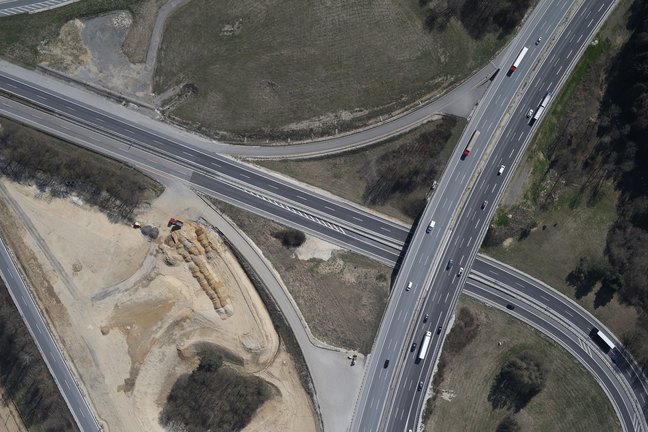
\includegraphics[width=0.45\textwidth]{L1234_rsz.png}
    \caption{\small Original Image}
    \label{fig:OriImg}
  }
  \quad
  \parbox{.475\linewidth}{
    \centering
    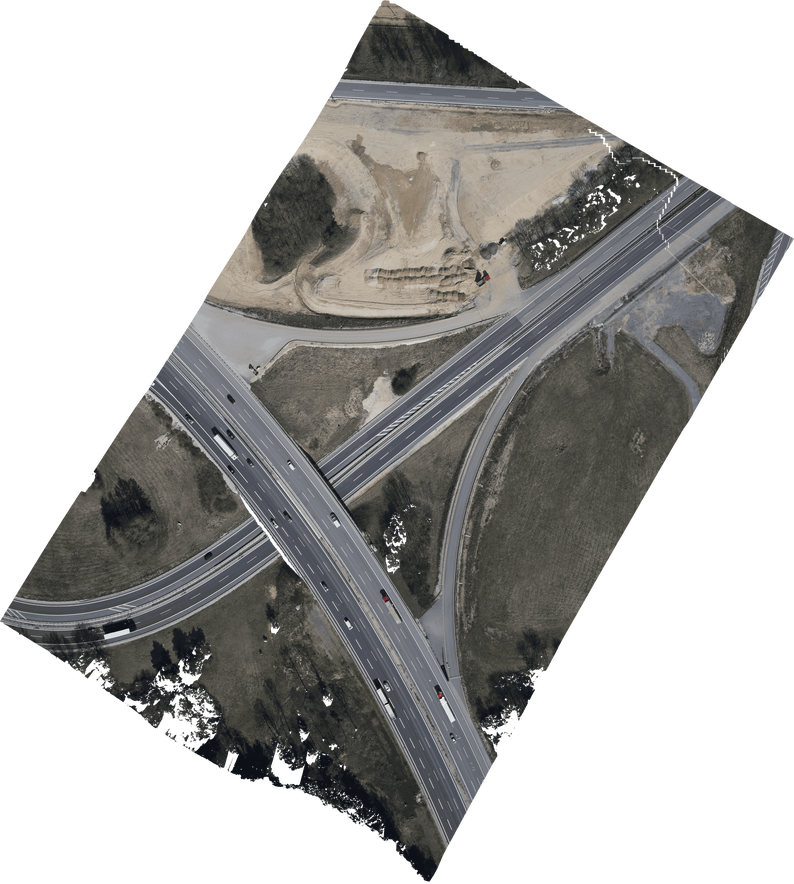
\includegraphics[width=0.45\textwidth]{OL1234_rsz.png}
    \caption{\small Orthorectified Image}
    \label{fig:OrthoImg}
  }
  \centering
  \parbox{.7\linewidth}{
    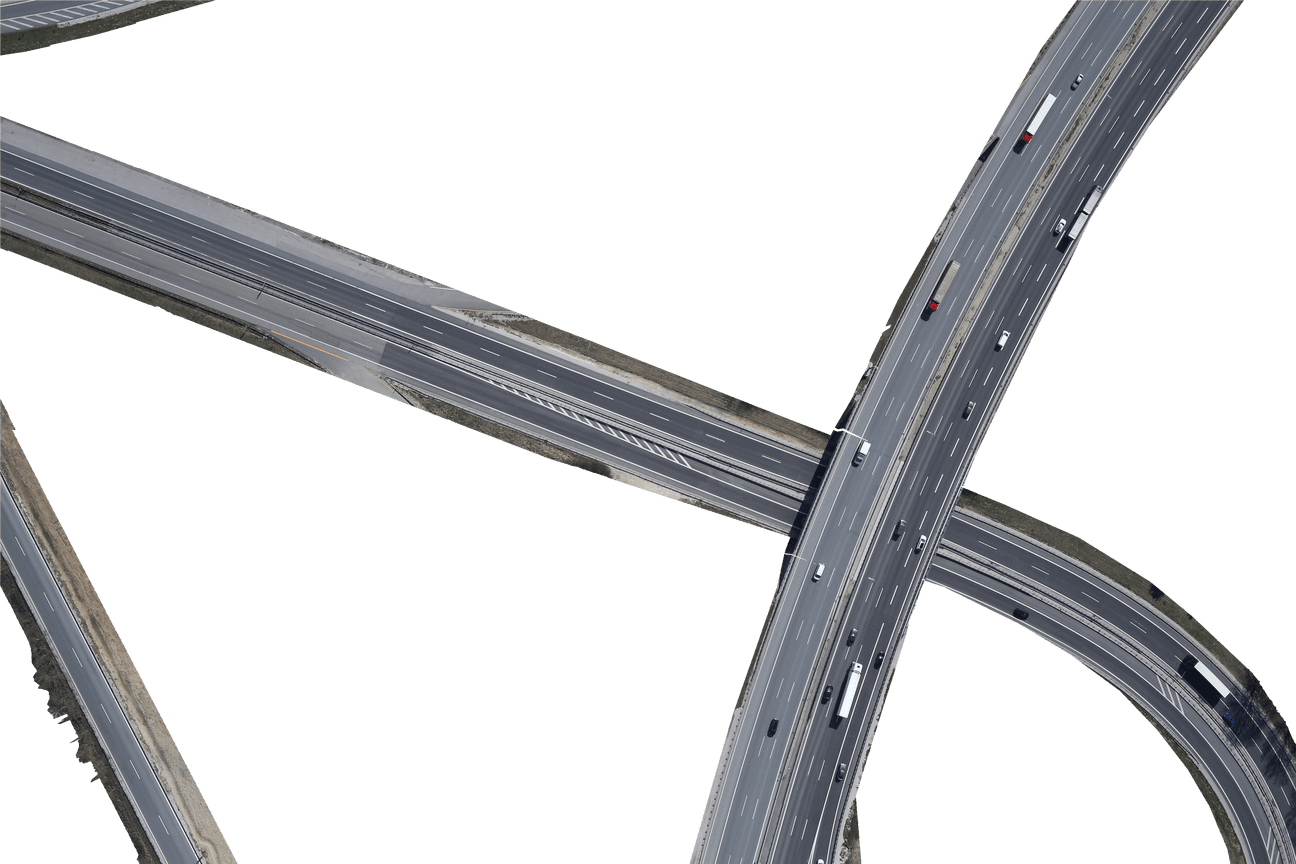
\includegraphics[width=0.7\textwidth]{ML1234_rsz.png}
    \caption{\small Masked Image}
    \label{fig:MaskedImg}
  }
\end{figure}

\clearpage
%%%%%%%%%%%%%%%%%%%%%%%%%%%%%%%%%%%%%%%%%%%%%%%%%%%%%%%%
\section{Preprocessing}
\label{sec:preprocessing}

In lane marking extraction step, the $\sigma$ value for Gaussian smoothing is set to be 1.8 % From HALCON Referenz: For the choice of the thresholds High and Low one has to keep in mind that the second directional derivative depends on the amplitude and width of the line as well as the choice of Sigma. Thus: you must set this value depending on the lane marking width?
to slightly suppress the noise in images.
The extracted lines of length less than 70 pixels are rejected % why
regarding the fact that a dashed lane-line is no longer than 6 meter which is correspondingly 87 pixels with GSD of 6.9 cm.
% http://www.mvtec.com/doc/halcon/11/en/lines_gauss.html
% https://www.dvr.de/download/publikationen-schriftenreihe-17.pdf

%%%%%%%%%%%%%%%%%%%%%%%%%%%%%%%%%%%%%%%%%%%%%%%%%%%%%%%%
\section{Simulation}
\label{sec:simulation}
This section aims to verify the correctness of the derived LS model using simulation data. The used materials are as described in \cref{sec:Materials}. Only the measurements (the image coordinates of the extracted lines), the true and approximate values of the unknowns (the object coordinates of a line segment) in the non-linear LS model are simulated, as described in \cref{subsec:simudata}.

Note that the quality of camera parameters (EO., IO. and additional parameters) do not have influences in simulation since the simulated measurements are produced with the same set of camera parameters as the set used for 3D reconstruction.

\cref{subsec:simuresult-1} aims to check if the iteration scheme converges to the correct solution given biased initial values of the unknowns. %\cref{subsec:simuresult-2} checks, without the influences from camera parameters' quality, if the derived LS model is able to resist the simulated random errors contained in the measurements.

table:
simu.case1: biased initial values of the unknowns
simu.case2: noisy measurements and biased initial values of the unknowns

covering images, observations, unknowns, redundancies, 



%1.random noise distribution

\subsection{Simulation Data}
\label{subsec:simudata}

\paragraph{The true line segment in object space}
Firstly, the object coordinates of the endpoints of a 3D line segment are defined, with 77 meter distance, locating on the road surface in the test area (German highway A9) with 7 aerial images coverage. By linear interpolating several points with 0.2 meter spaces (considering DSM grid of 0.2 meter) between the two endpoints, a 3D line segment in the form of a set of 3D points is generated .
The location of this 3D line segment serves as the true values in the experiments in this subsection. 

\paragraph{The observed line segments in image spaces}
The observations in the LS model are simulated by back-projecting the true line segment into the covering images. No noise is added in the observations.

\paragraph{The approximate line segment in object space}
The initial estimates for non-linear LS adjustment is generated by %projecting the true line segment onto the DSM and additionally 
adding some known biases in the coordinates of the true line segment's endpoints.
\begin{table} [h!]
  \centering
  \begin{tabular}{l|lll|lll}
  \toprule
                         & \multicolumn{3}{c}{start-point} & \multicolumn{3}{|c}{end-point}\\
                         & $X_s$    & $Y_s$    & $Z_s$       & $X_e$    & $Y_e$    & $Z_e$\\
  \midrule
  the added bias [meter] & $0$      & $0$      & $+0.5$      & $+0.2$   & $+0.1$   & $+0.3$\\
  \bottomrule
  \end{tabular}
  \caption{The added biases in the object coordinates of the true line segment's endpoints. I.e. they are the known biases added in the unknown parameters in the LS adjustment.}
  \label{tab:BiasesInInitialValues}
\end{table}

\subsection{Simulation Result}
\label{subsec:simuresult}

%%% analysis on measurements:
% 1.residuals distribution: histogram (fit line: mean, standard deviation)
% 2.normal distribution? systematic error exist? statistical test
%   or
%   standard deviation small enough? statistical test

%statistical test: errors small enough?

%%% analysis on the unknowns:
\cref{fig:Simu3D_2} shows the reconstructed and the true line segments in UTM coordinate system (in Zone 32N). The distances from the reconstructed line segment to the true one are plotted into histogram in \cref{fig:SimuHist_2}. They are sampled along the reconstructed line with 0.2 meter spacing, resulting in sample size of 385. The sample mean is -0.001 [meter] and the sample standard deviation is 0.016 [meter].

To test if the population mean significantly equals zero, t-test is adopted. With null hypothesis($H_0$) and (two-tailed) alternative hypothesis ($H_A$) being stated as:
\begin{equation}
\begin{split}
H_0: \mu=\overline{x}\\
H_A: \mu\neq\overline{x}
\end{split}
\end{equation}

With the sample mean $\overline{x}=-0.001$,
the proposed population mean $\mu=0$,
the sample standard deviation $s=0.016$,
and sample size $n=385$, the test statistic $T$ for a One Sample t Test has a calculated value:
\begin{equation}
T_{obs} = \frac{\overline{x} - \mu_0}{s/\sqrt{n}}=\frac{-0.001-0}{0.016/\sqrt{385}}\approx1.226
\end{equation}

A selected significance level $\alpha=0.05$ with degree of freedom $dof=385-1=384$ leads to the critical t-value $T_{cri}=1.660$ (from t Table). As the observed value $T_{obs}=1.226$ is not in the critical region, we fail to reject the null hypothesis. In other words, with 95\% confidence we can claim that the sample mean value of the distances from the reconstructed line segment to the true line segment equals to 0.


The mean  is zero (statistical test).


\clearpage
reconstructed line vs true line (accuracy?)

\begin{figure} [h!]
%  \parbox{.475\linewidth}{
%  }
  \centering
  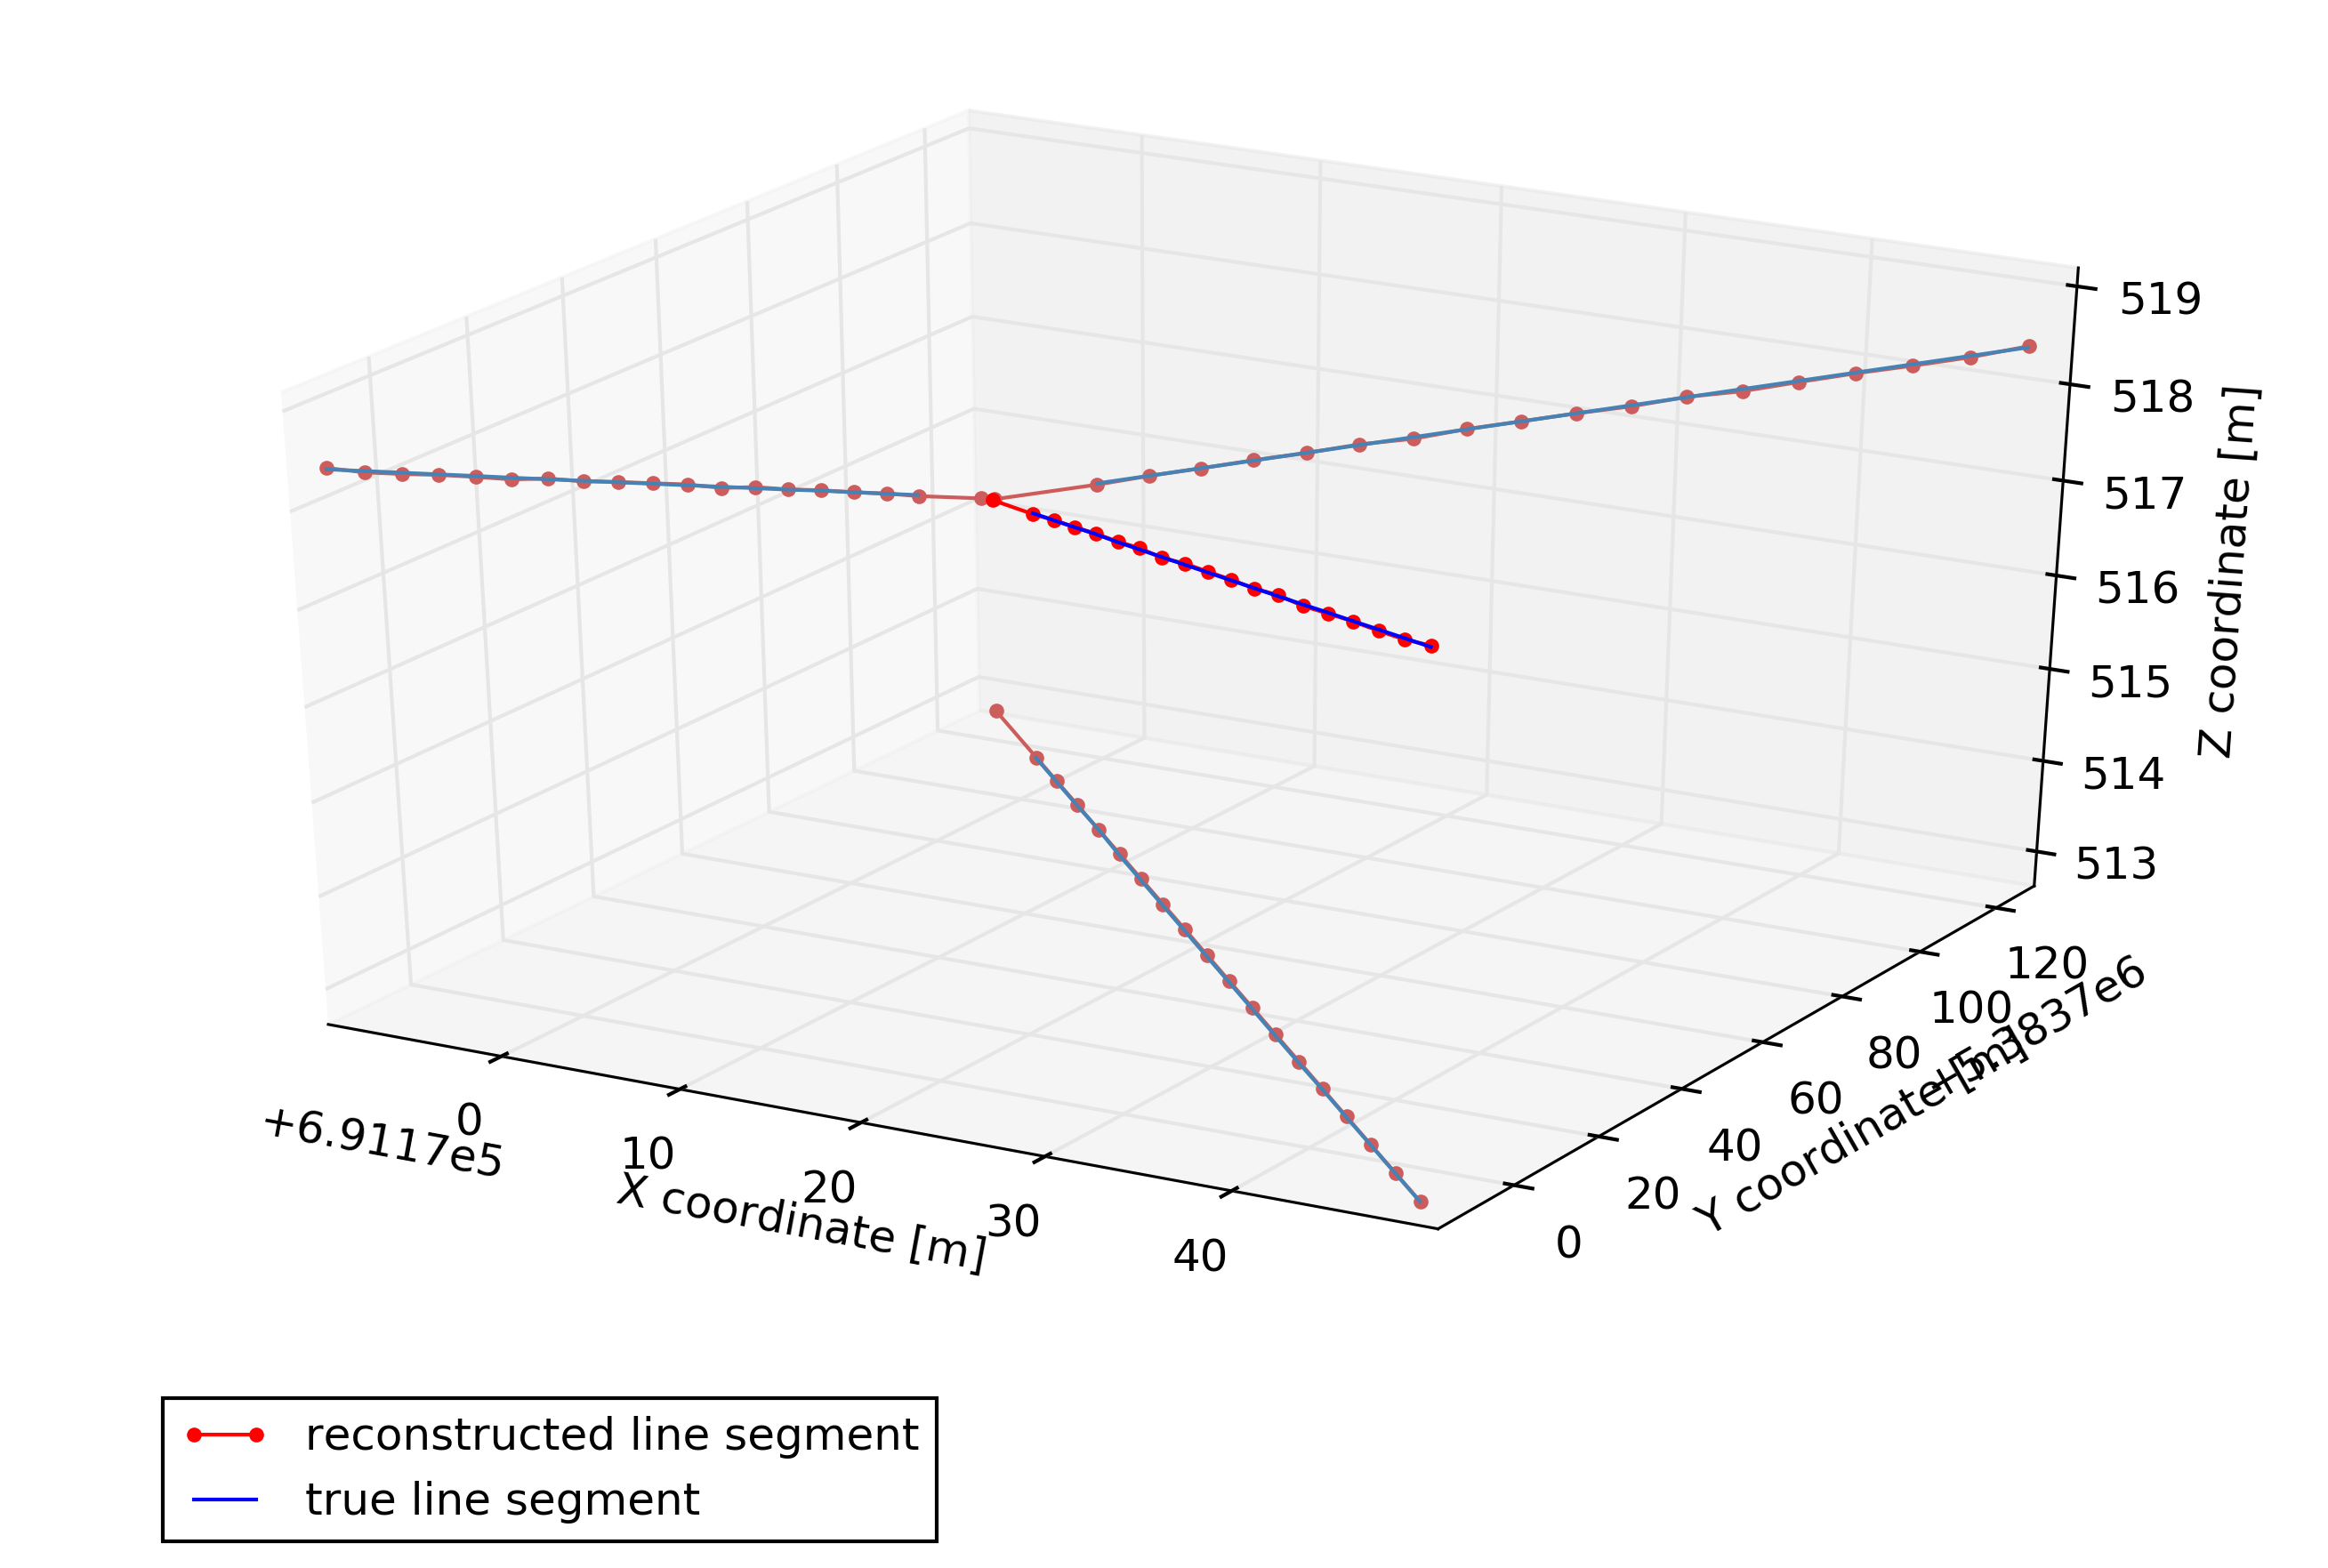
\includegraphics[width=0.9\textwidth]{Simu_3D_2.png} %%% 換,字重疊、圖例太右下。
  \caption{\small The reconstructed line and the true line.}
  \label{fig:Simu3D_2}
  \vspace{1cm}
  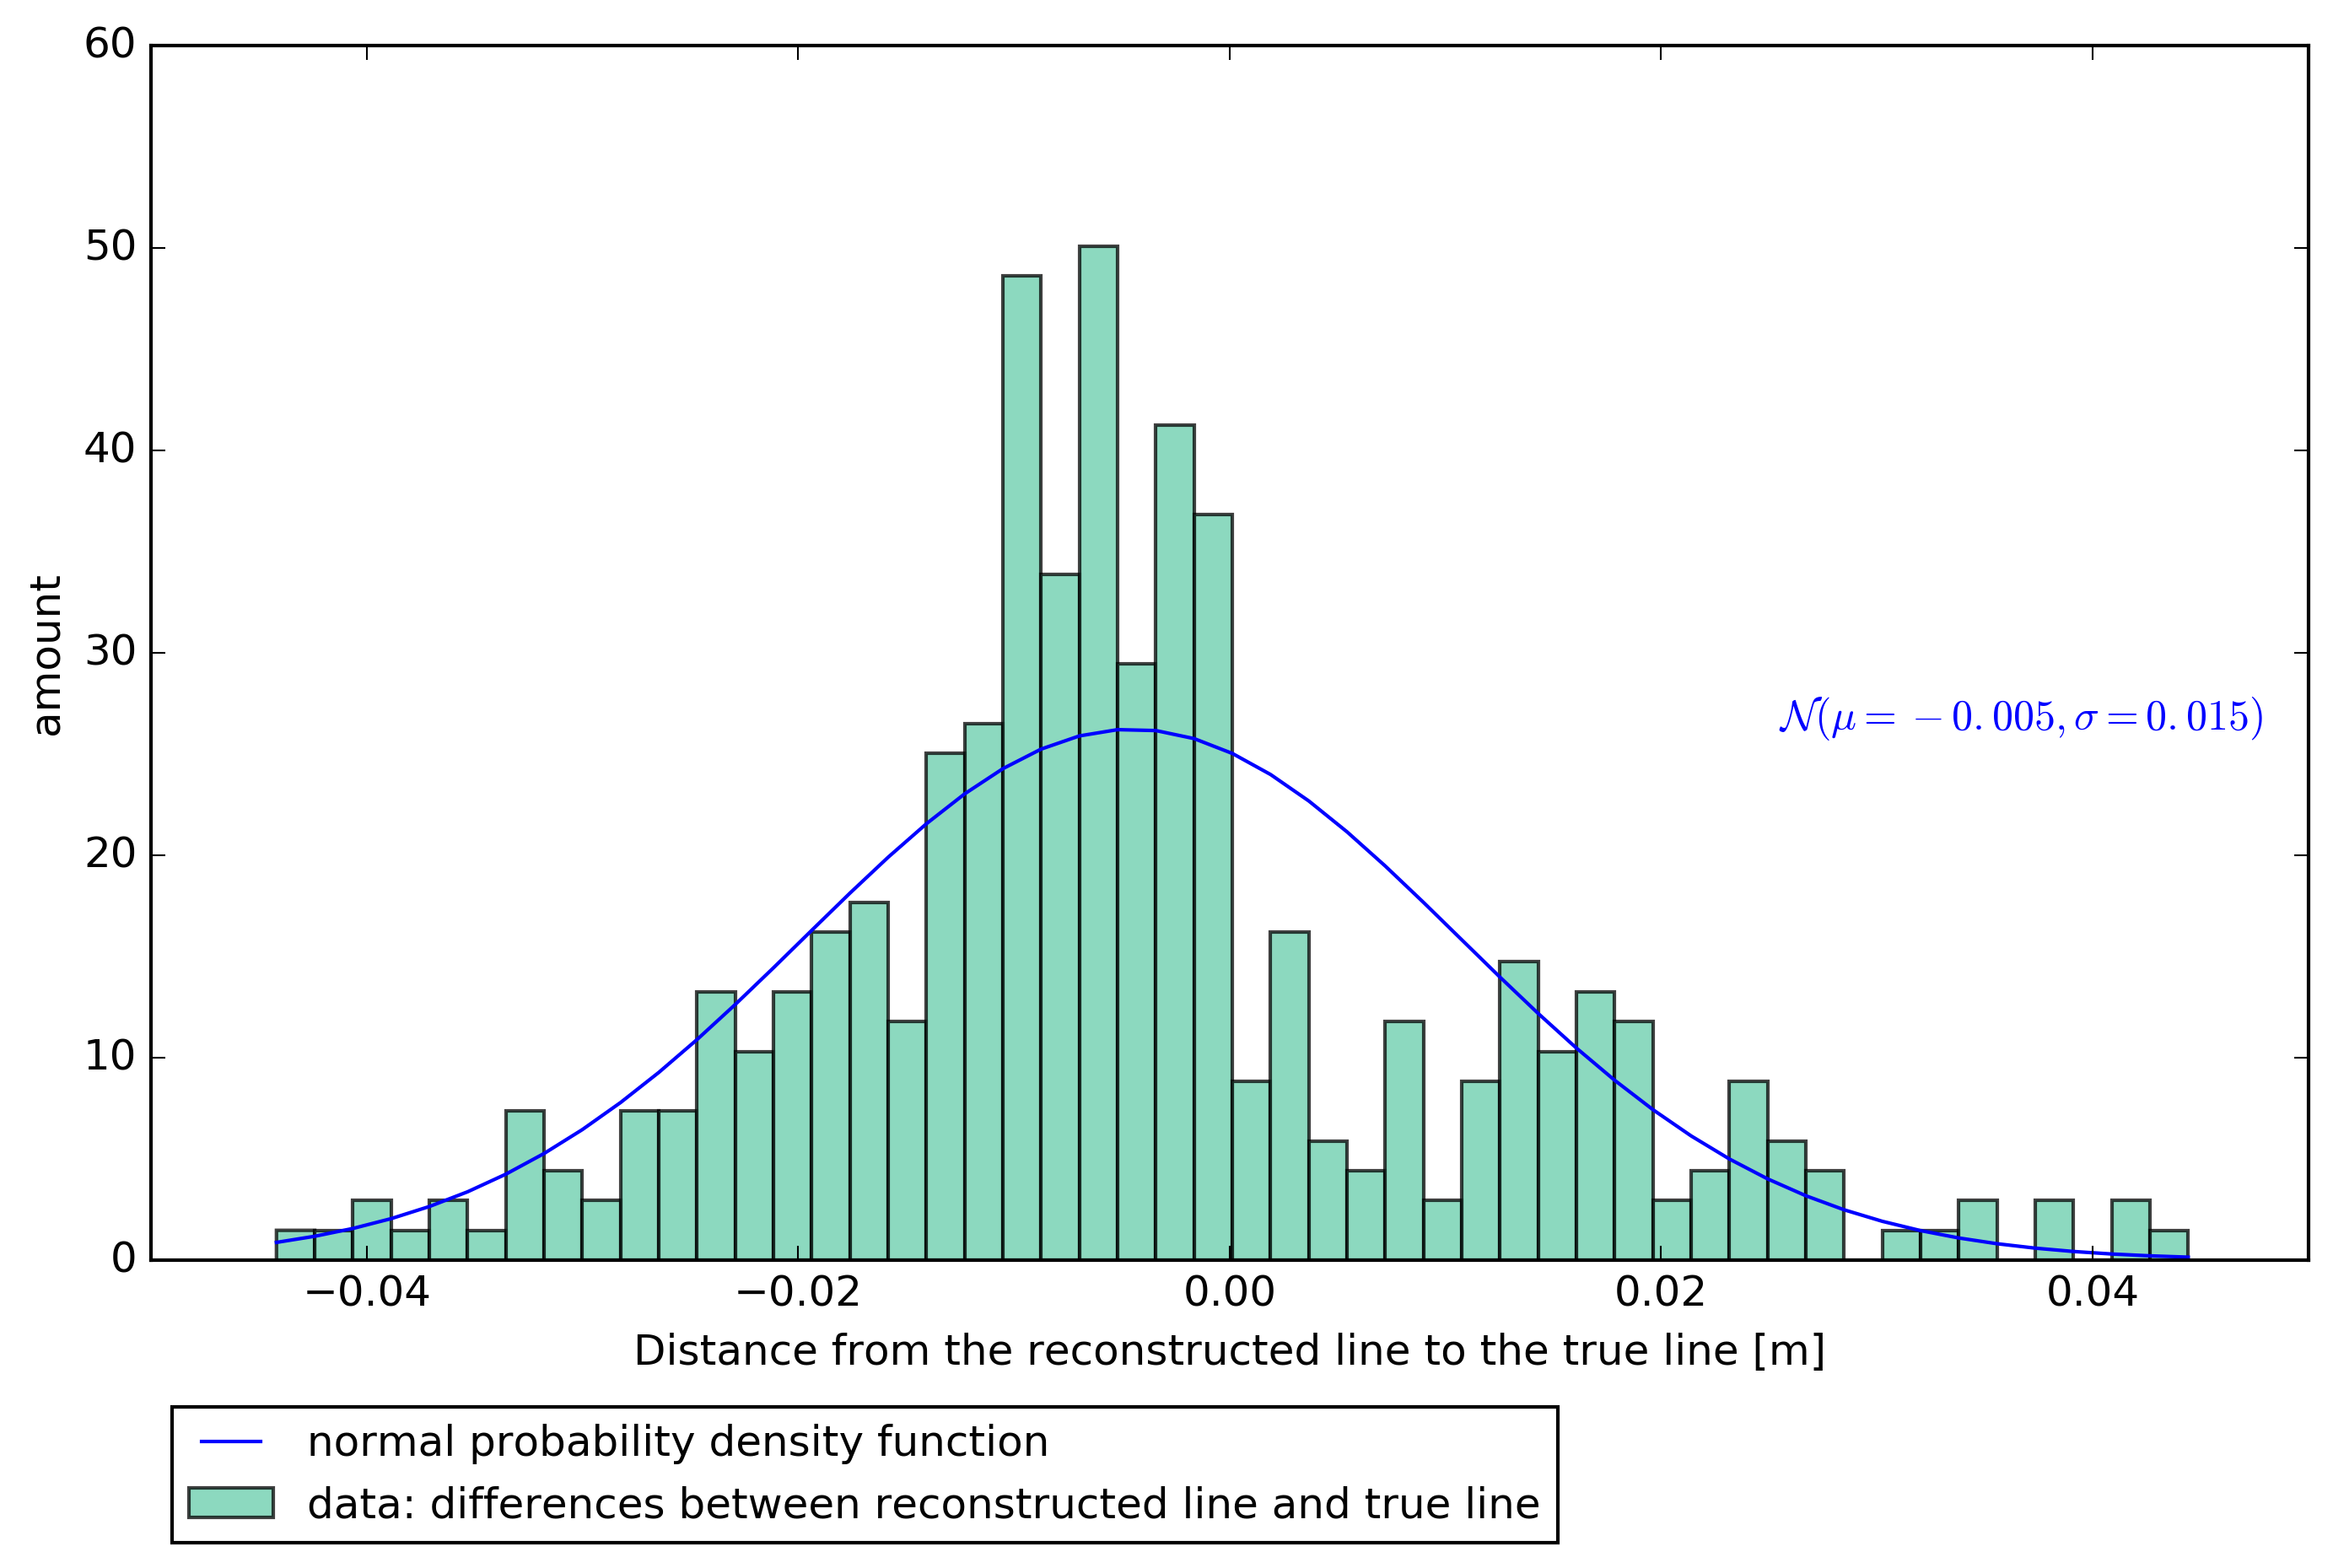
\includegraphics[width=0.8\textwidth]{Simu_hist_2.png} %%% 換,字太小。
  \caption{\small Histogram of the distances between the reconstructed line and the true line.}
  \label{fig:SimuHist_2}
\end{figure}





\clearpage
reconstructed line vs unrefined DSM profile line (accuracy?)
\begin{figure} [h!]
%  \parbox{.475\linewidth}{
%  }
  \centering
  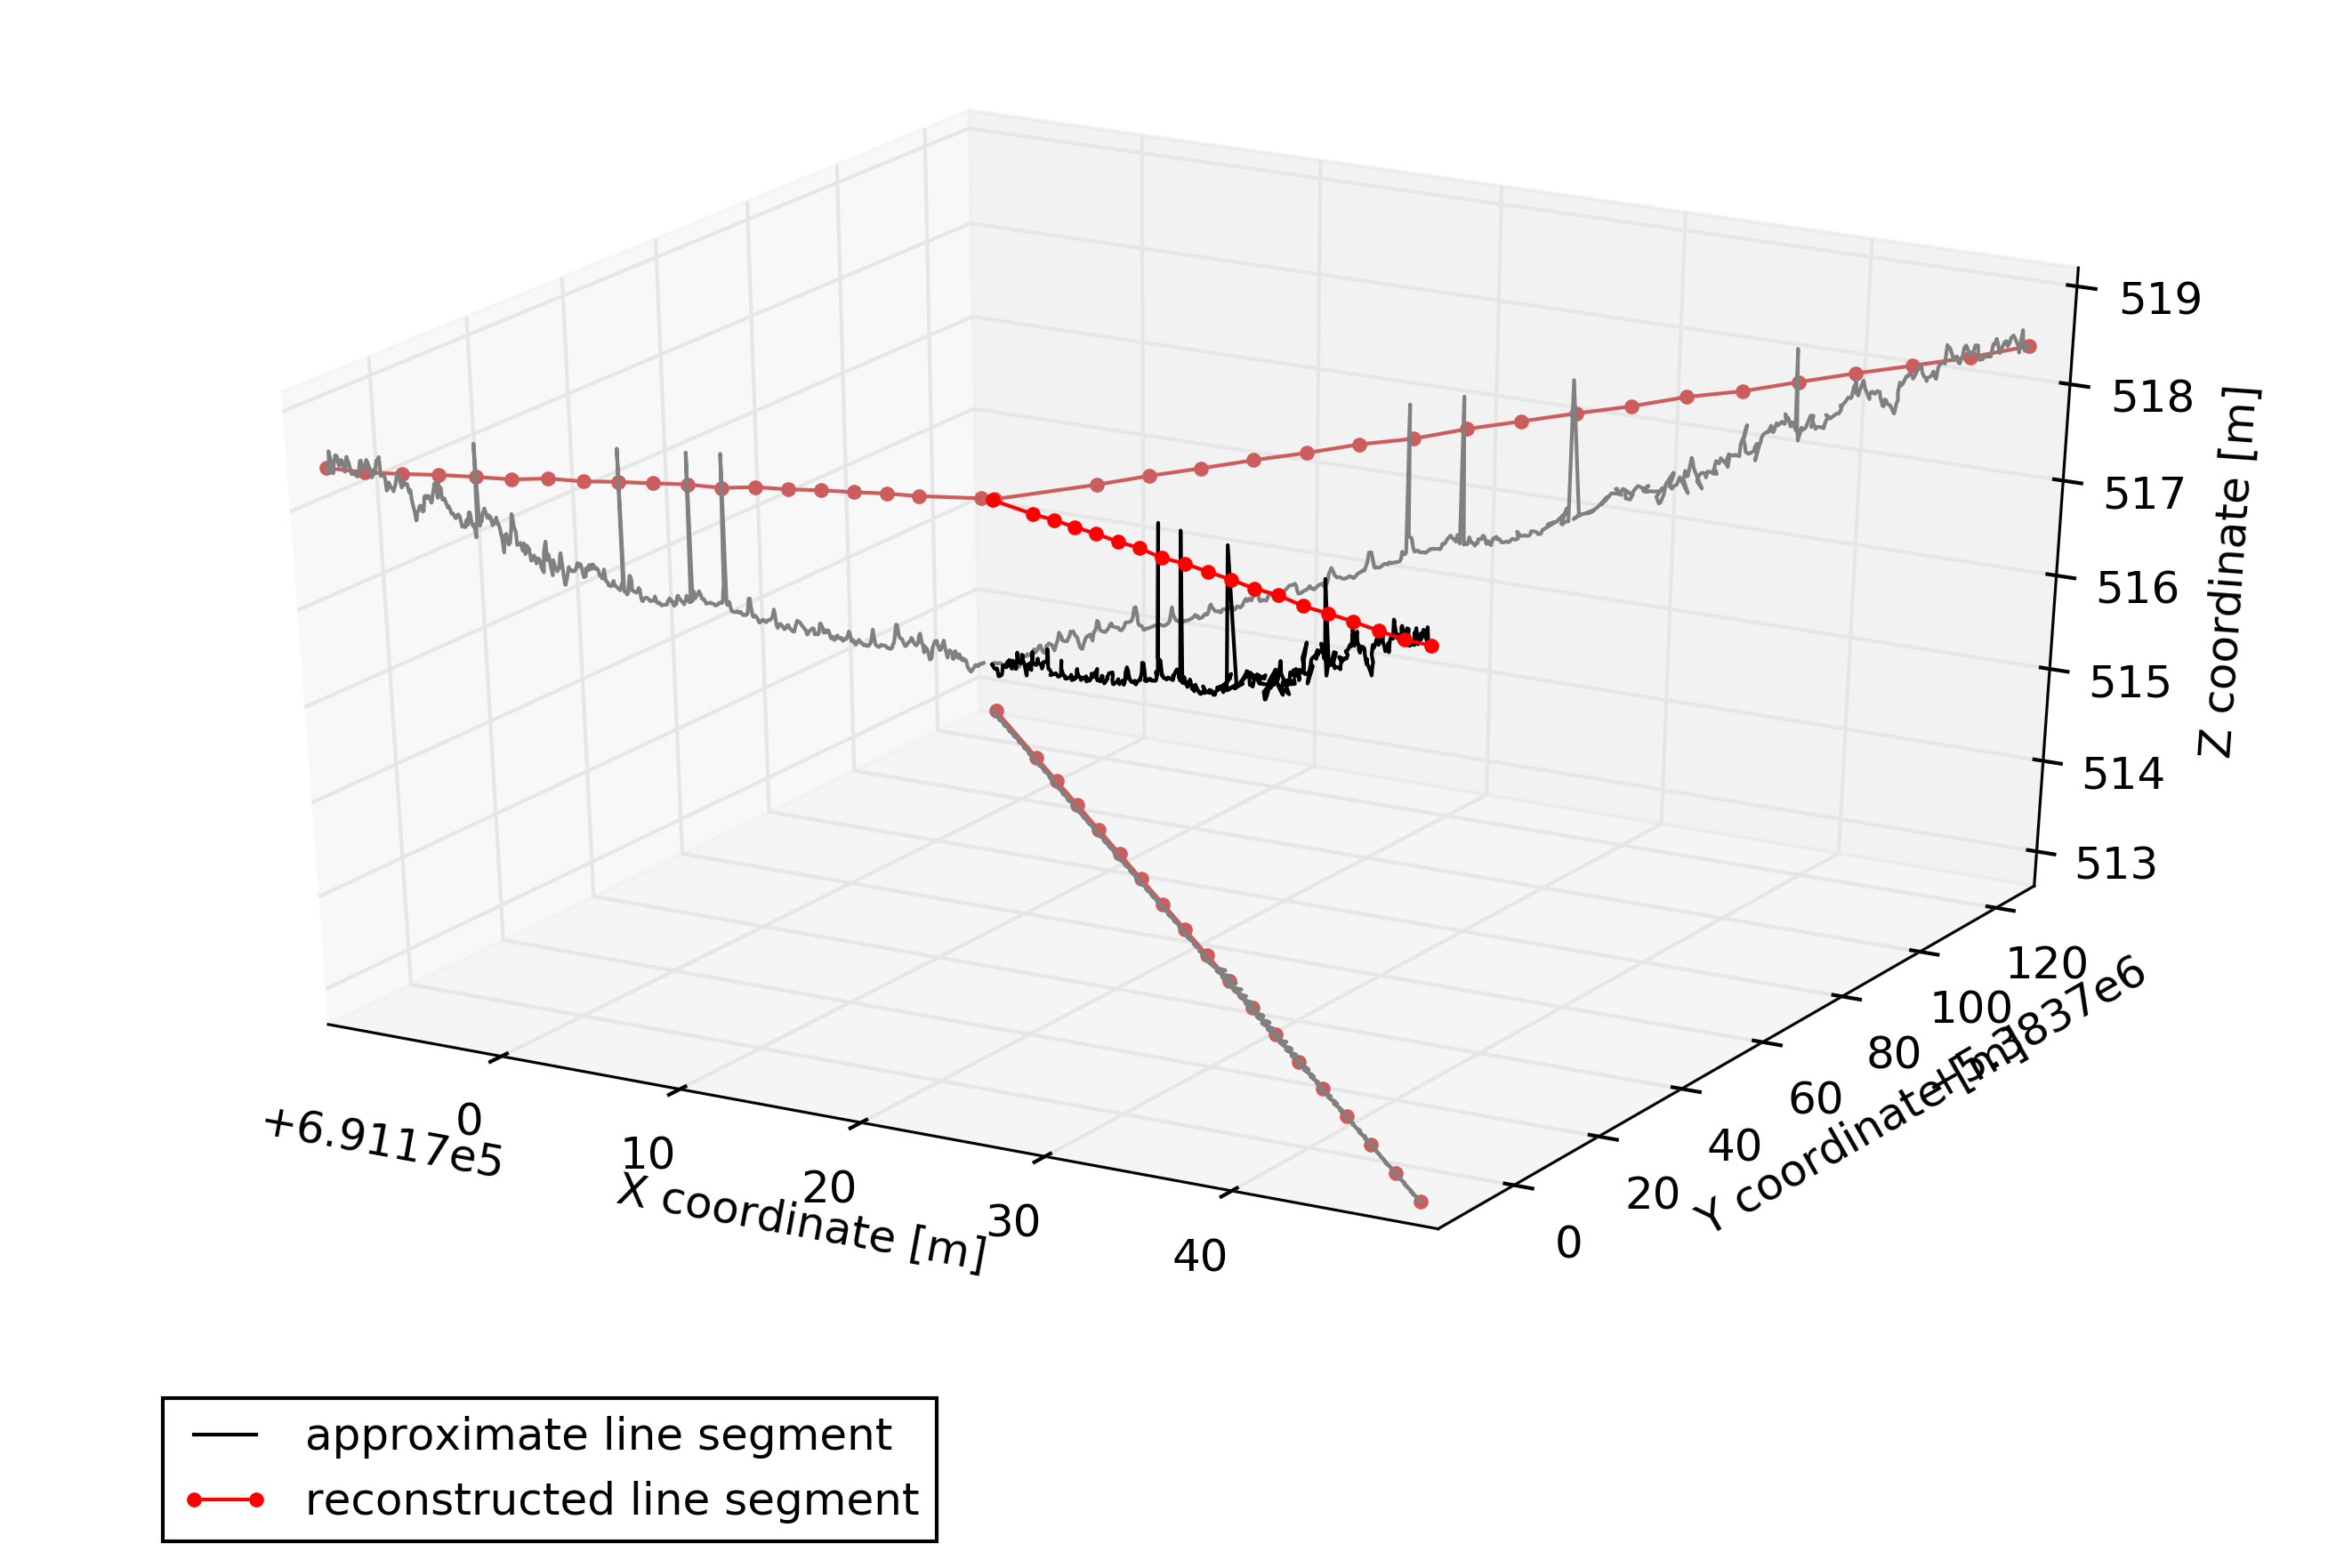
\includegraphics[width=0.9\textwidth]{Simu_3D_1.png} %%% 換,字重疊、圖例太右下。
  \caption{\small The reconstructed line and the unrefined DSM profile.}
  \label{fig:Simu3D_1}
  \vspace{1cm}
  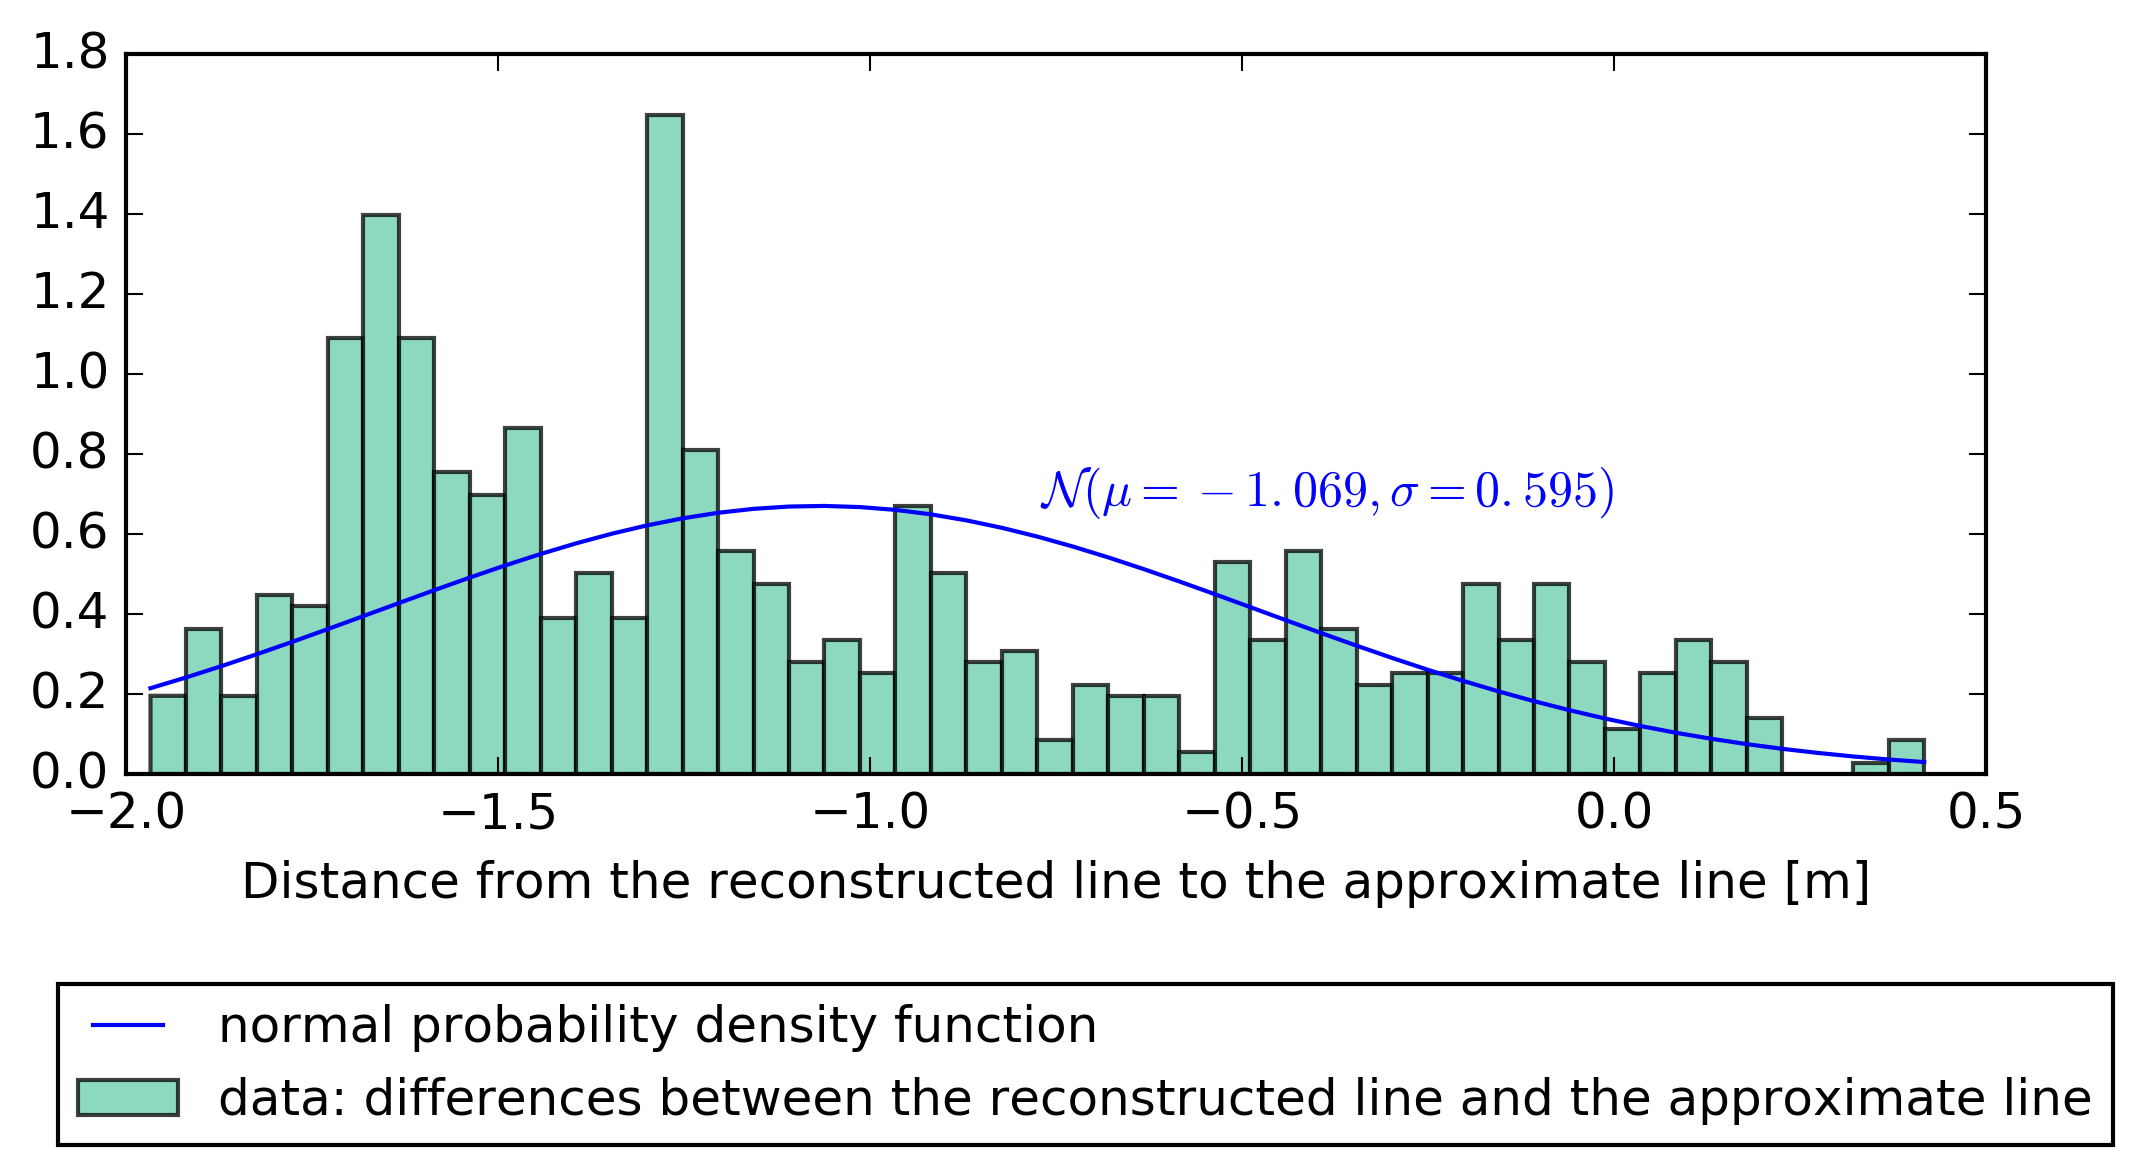
\includegraphics[width=0.8\textwidth]{Simu_hist_1.png} %%% 換,字太小。
  \caption{\small Histogram of the distances between the reconstructed line and the unrefined DSM profile.}
  \label{fig:SimuHist_1}
\end{figure}

analysis on the unknowns:

\cref{fig:Simu3D_1} shows the reconstructed line segments and the unrefined DSM profile in UTM coordinate system (in Zone 32 ??). The distance from the reconstructed line segment to the approximation

the differences appears non-normal distributed and the first moment is non-zero/ negative (proved by statistical test)

This phenomenon is as expected, as mentioned in sec:DSM??? 




\clearpage



%\subsection{Simulation Result: case 2}
%\label{subsec:simuresult-2}
%analysis on measurements:
% 1.residuals distribution: histogram (fit line: mean, standard deviation)
% 2.normal distribution? systematic error exist? statistical test
% 3.as expected? (the same as the added random errors) statistical test
 
%reconstructed line vs true line (accuracy?)

%statistical test: errors small enough?




%%%%%%%%%%%%%%%%%%%%%%%%%%%%%%%%%%%%%%%%%%%%%%%%%%%%%%%%
\section{True Data}
\label{sec:truedata}

table:
case1: Dashed Lane marking
case2: Continuous Lane marking%, two strips, multiple stereo pairs
%case3: Continuous Lane marking, two strips, two stereo pairs
%case4: Continuous Lane marking, two strips, one stereo pair
%case5: Continuous Lane marking, one strip

covering images, observations, unknowns, redundancies, 



\subsection{True Data Result: case 1 -Dashed Lane Marking}
\label{subsec:trueresult-1}


\subsection{True Data Result: case2 -Continuous Lane Marking}
\label{subsec:trueresult-2}


\begin{figure} [h!]
%  \parbox{.475\linewidth}{
%  }
  \centering
  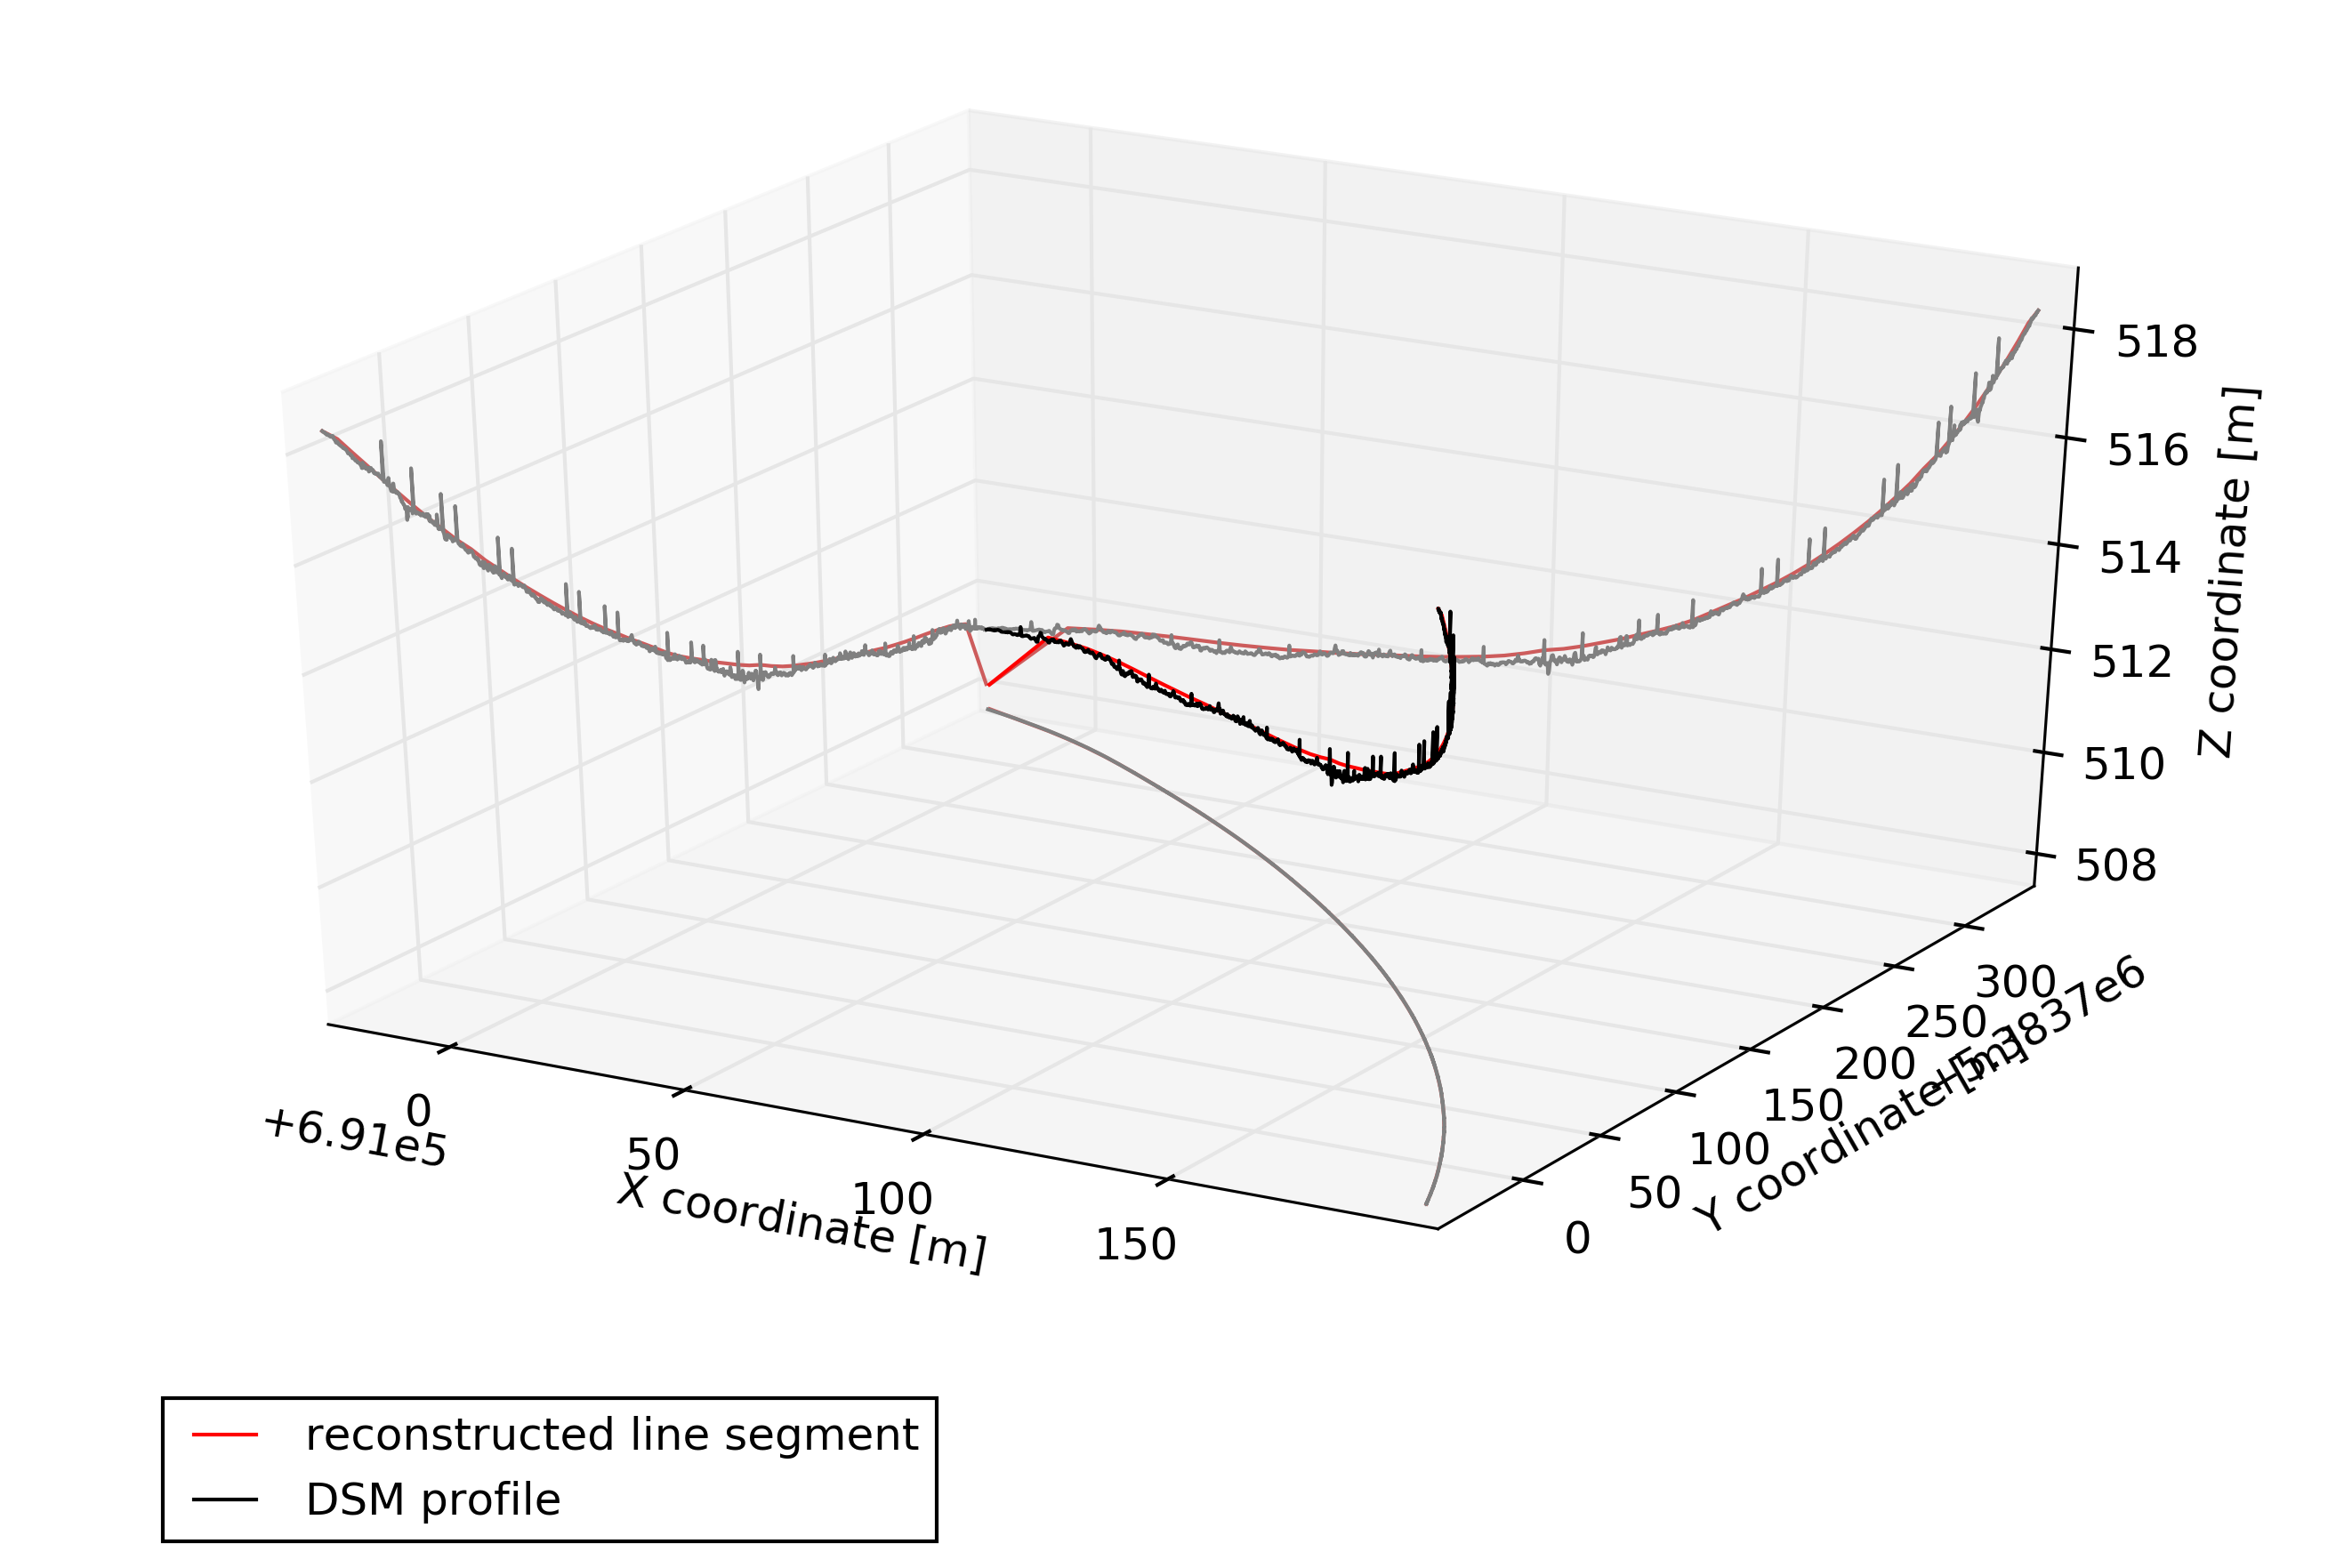
\includegraphics[width=0.9\textwidth]{Test_3D_1.png} %%% 換,字重疊、圖例太右下。
  \caption{\small The reconstructed line and the unrefined DSM profile.}
  \label{fig:Test3D_1}
  \vspace{1cm}
  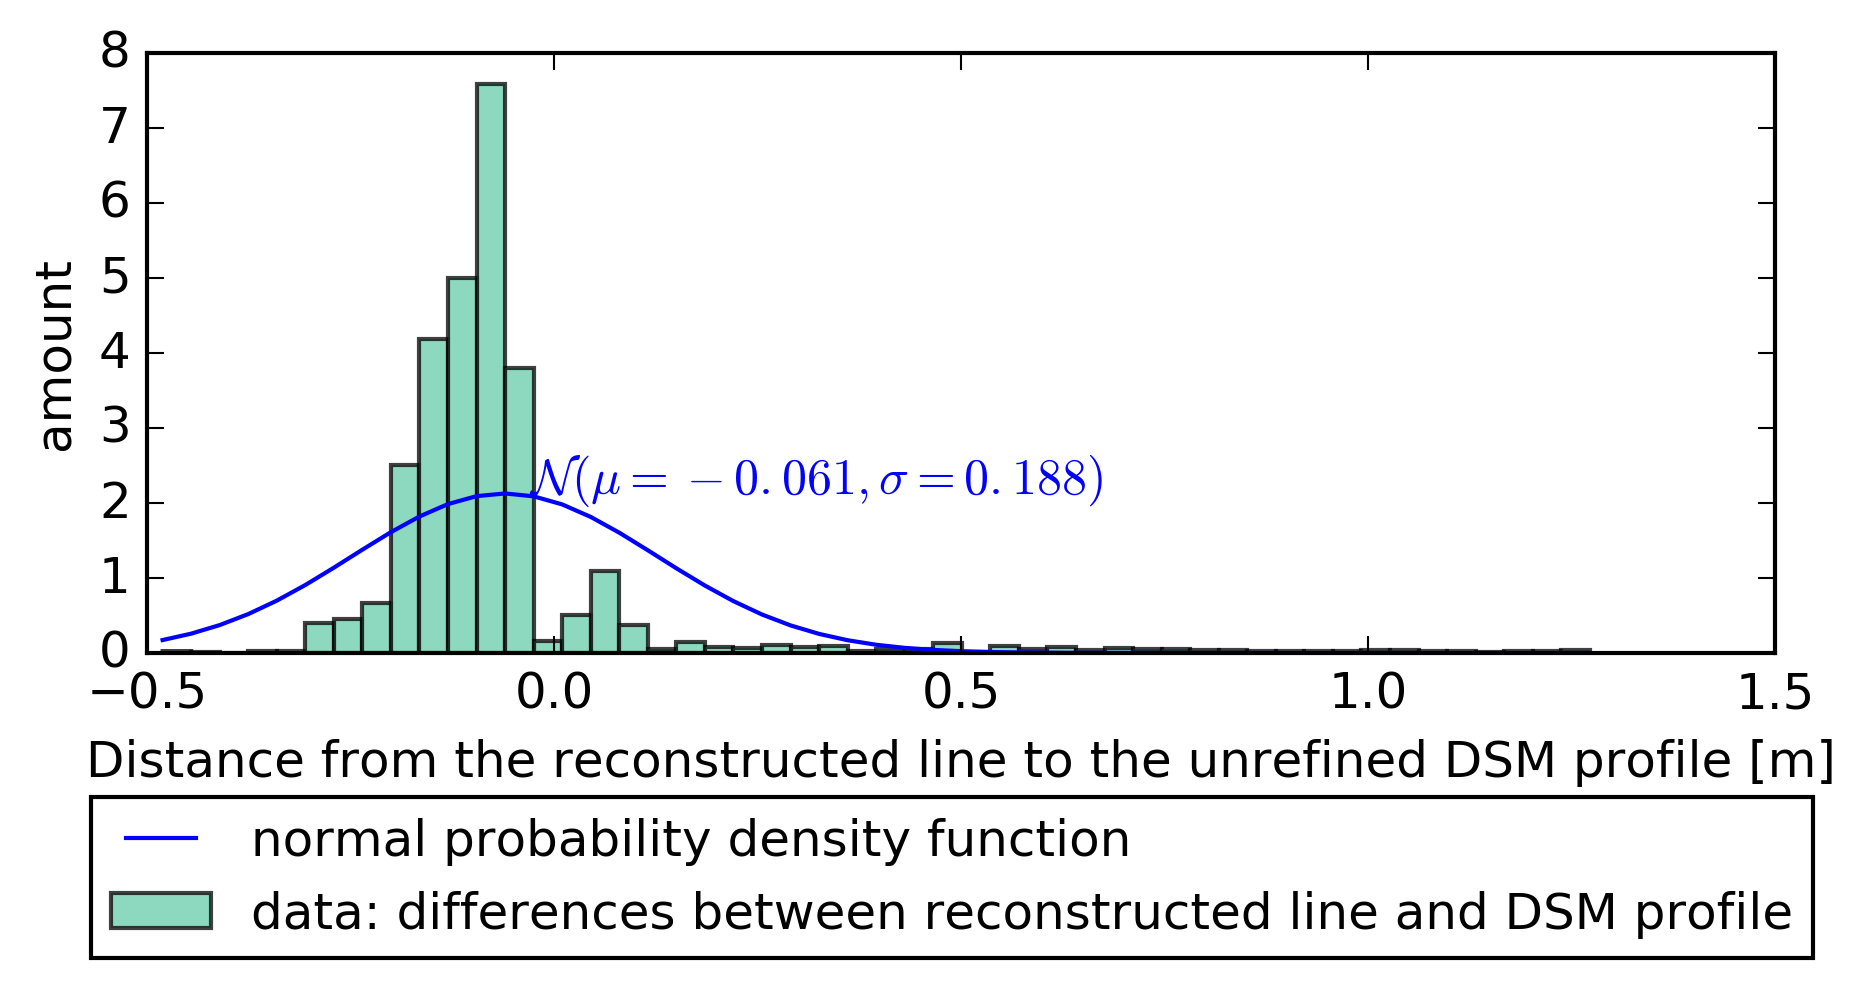
\includegraphics[width=0.8\textwidth]{Test_hist_1.png} %%% 換,字太小、增加xtick。
  \caption{\small Histogram of the distances between the reconstructed line and the unrefined DSM profile.}
  \label{fig:TestHist_1}
\end{figure}

analysis on unknowns:
of 453.6 meter
The DSM profile is in average 6 cm lower than the reconstructed line. 


%\subsection{True Data Result: case2-5}
%\label{sec:trueresult-3}




%%%%%%%%%%%%%%%%%%%%%%%%%%%%%%%%%%%%%%%%%%%%%%%%%%%%%%%%
\section{Discussion: Influence of the Image Distribution and Amount}
\label{sec:discussion-ImageDistributionAmount}




%%%%%%%%%%%%%%%%%%%%%%%%%%%%%%%%%%%%%%%%%%%%%%%%%%%%%%%%
%3.1  Reference Data
%The primary reference dataset used in this paper is a 3D point cloud acquired by airborne laser scanning with a density of approximately 0.5 points per square meter.  The laser point cloud data is georeferenced in UTM Zone 31 North, ETRS89 and contains orthometric heights with respect to EGM 2008.  The orthometric  heights  were  converted  to  ellipsoidal  heights  by  simply dding the undulations from EGM 2008.  Only the first pulse returns is used in this study, as the DSM produced by image matching corresponds to the visible surface.  The LIDAR data for the errassa and Vacarisses test areas was acquired on 26th and 27th ovember 2007. The LaMola LIDAR data was acquired on 26th ovember 2007 and 4th May 2008

%%%%%%%%%%%%%%%%%%%%%%%%%%%%%%%%%%%%%%%%%%%%%%%%%%%%%%%%
4.3 Internal Factors

4.3.1 Correctness of

4.3.2 Verification of

4.3.3 Precision of


%%%%%%%%%%%%%%%%%%%%%%%%%%%%%%%%%%%%%%%%%%%%%%%%%%%%%%%%
4.4 External Factors

4.4.1 Influence of 

%noch etwas Fülltext
%\blinddocument
